After the process of feature selection was completed parameter training by means of Stochastic Gradient Descent could take place. Values of the trained weights are presented in Table \ref{table:weights_nonlinear_noise_free}.
\npdecimalsign{.}
\nprounddigits{5}
\begin{table}[ht]
\caption{Trained weights for segmentation of noise free images.}
\centering
\begin{tabular}{|c|c|c|}
\hline
\rowcolor[HTML]{C0C0C0} 
$w_1$(unary potential) & $w_{2,1}$ (pairwise potential) & $w_{2,2}$ (bias) \\ \hline
0.11973 & 1.00649 & 0.38711 \\ \hline
\end{tabular}
\label{table:weights_nonlinear_noise_free}
\end{table}

Having a model parametrised with those weights it was possible to perform inference on the set of unknown test samples. Figure \ref{fig:nonlinear_results_noise_free} presents the results of the semantic segmentation process on sample test images. In the first column an original image that is to be segmented is showed and in the second this image after the process of colour quantisation. The next two columns depict segmentation results, one with only local potential, and the second one with both potentials involved. The last column presents the expected results.  
\begin{figure}[!htb]
 \centering
 \setlength{\tabcolsep}{2pt}
    \begin{tabular}{m{0.19\textwidth}m{0.19\textwidth}m{0.19\textwidth}
    m{0.19\textwidth}m{0.19\textwidth}}
    \thead{sample \\ image} & \thead{colour \\ quantisation} & \thead{local \\ potential} & \thead{experimental \\ result} & \thead{expected \\ result} \\ 
       \fcolorbox{black}{white}{\includegraphics[width = 0.19\textwidth]{nonlinear_noise_free/experiments/init/17.png}} &
       \fcolorbox{black}{white}{\includegraphics[width = 0.19\textwidth]{nonlinear_noise_free/experiments/quant/17.png}} &
       \fcolorbox{black}{white}{\includegraphics[width = 0.19\textwidth]{nonlinear_noise_free/experiments/only_fi1/17.png}} &
        \fcolorbox{black}{white}{\includegraphics[width = 0.19\textwidth]{nonlinear_noise_free/experiments/results/17.png}} &
        \fcolorbox{black}{white}{\includegraphics[width = 0.19\textwidth]{nonlinear_noise_free/experiments/ground_truth/17.png}} \\
        %
        \fcolorbox{black}{white}{\includegraphics[width = 0.19\textwidth]{nonlinear_noise_free/experiments/init/19.png}} &
        \fcolorbox{black}{white}{\includegraphics[width = 0.19\textwidth]{nonlinear_noise_free/experiments/quant/19.png}} &
        \fcolorbox{black}{white}{\includegraphics[width = 0.19\textwidth]{nonlinear_noise_free/experiments/only_fi1/19.png}} &
        \fcolorbox{black}{white}{\includegraphics[width = 0.19\textwidth]{nonlinear_noise_free/experiments/results/19.png}} &
        \fcolorbox{black}{white}{\includegraphics[width = 0.19\textwidth]{nonlinear_noise_free/experiments/ground_truth/19.png}} \\
        %
        \fcolorbox{black}{white}{\includegraphics[width = 0.19\textwidth]{nonlinear_noise_free/experiments/init/20.png}} &
        \fcolorbox{black}{white}{\includegraphics[width = 0.19\textwidth]{nonlinear_noise_free/experiments/quant/20.png}} &
        \fcolorbox{black}{white}{\includegraphics[width = 0.19\textwidth]{nonlinear_noise_free/experiments/only_fi1/20.png}} &
        \fcolorbox{black}{white}{\includegraphics[width = 0.19\textwidth]{nonlinear_noise_free/experiments/results/20.png}} &
        \fcolorbox{black}{white}{\includegraphics[width = 0.19\textwidth]{nonlinear_noise_free/experiments/ground_truth/20.png}} \\
        %
        \fcolorbox{black}{white}{\includegraphics[width = 0.19\textwidth]{nonlinear_noise_free/experiments/init/23.png}} &
        \fcolorbox{black}{white}{\includegraphics[width = 0.19\textwidth]{nonlinear_noise_free/experiments/quant/23.png}} &
        \fcolorbox{black}{white}{\includegraphics[width = 0.19\textwidth]{nonlinear_noise_free/experiments/only_fi1/23.png}} &
        \fcolorbox{black}{white}{\includegraphics[width = 0.19\textwidth]{nonlinear_noise_free/experiments/results/23.png}} &
        \fcolorbox{black}{white}{\includegraphics[width = 0.19\textwidth]{nonlinear_noise_free/experiments/ground_truth/23.png}} \\
        %
        \fcolorbox{black}{white}{\includegraphics[width = 0.19\textwidth]{nonlinear_noise_free/experiments/init/7.png}} &
        \fcolorbox{black}{white}{\includegraphics[width = 0.19\textwidth]{nonlinear_noise_free/experiments/quant/7.png}} &
        \fcolorbox{black}{white}{\includegraphics[width = 0.19\textwidth]{nonlinear_noise_free/experiments/only_fi1/7.png}} &
        \fcolorbox{black}{white}{\includegraphics[width = 0.19\textwidth]{nonlinear_noise_free/experiments/results/7.png}} &
        \fcolorbox{black}{white}{\includegraphics[width = 0.19\textwidth]{nonlinear_noise_free/experiments/ground_truth/7.png}} \\
    \end{tabular}
    \caption{Experimental results of shape-based semantic image segmentation on noise-free images.}
    \label{fig:nonlinear_results_noise_free}
\end{figure}

As presented, the semantic segmentation on the test set of images that was based on the new definition of the feature function was much more successful. Objects with a shape of the letter H were properly assigned to the class of label 3 and distinguished from other red objects, which belong to class 0. Green regions have label 1 and blue label 2, just as expected. When it comes to the comparison between the results obtained with local potential only, and final results, by including a pairwise potential the accuracy of the performed segmentation was improved. It is especially visible on individual pixels on object boundaries, which were assigned to an incorrect class by local potential but are correctly labelled in a final result. The last row of Figure \ref{fig:nonlinear_results_noise_free} shows a large improvement after addition of the local potential. A green superpixel at the bottom right corner of surroundings of the letter H had his labelling improved. Furthermore, also a classification of a group of four red superpixels that were incorrectly assigned to class 3, was corrected by using a full energy function. However, not in all cases did the pairwise potential manage to improve wrong labellings. It is especially visible in narrow, vertical, red regions surrounded only by green and red superpixels. In such cases the system confuses them with a vertical stripe of the letter H and incorrectly assigns them to class 3. Tough, the final results shows some improvement comparing to the results of a local potential only, not every superpixel has a correct labelling. The final accuracy of the described method on a set of test images expressed in terms of Intersection over Union is presented in Table \ref{table:iou_nonlinear_noise_free}. 
\begin{table}[ht]
\centering
\caption{Accuracy of segmentation based on shape detection for noise free data.}
\label{table:iou_nonlinear_noise_free}
    \begin{tabular}{|
    >{\columncolor[HTML]{9B9B9B}}c|c|c|c|c|
    >{\columncolor[HTML]{343434}}c|}
    \hline
    \textit{class} & \cellcolor[HTML]{9B9B9B}label 0 & \cellcolor[HTML]{9B9B9B}label 1 & \cellcolor[HTML]{9B9B9B}label 2 &  \cellcolor[HTML]{9B9B9B}label 3 & {\color[HTML]{FFFFFF} mIoU {[}\%{]}} \\ \hline
    local potential IoU {[}\%{]} & 97.89 & 99.95 & 99.91 & 95.51  &{\color[HTML]{FFFFFF} 98.32} \\ \hline
    final IoU {[}\%{]} & 99.32 & 100.00 & 100.00 & 98.84 &{\color[HTML]{FFFFFF} 99.54} \\ \hline
    \end{tabular}
\end{table}
As shown, after including the pairwise potential the accuracy of labellings for class 1 and 2 is equal to 100\%. Classification of object with the shape of the letter H has the lowest accuracy, tough it is still on a level of 98.84\%. Mean Intersection over Union over all labels for this this experiment was equal to 99.54\%. In general, addition of a pairwise potential improved the final precision of the segmentation process by 1.22 percent points.